\newpage
\appendix
\section{Glossary, abbreviations and acronyms}
\label{sec:appendix-glossary}
\begin{description}
\item[AOD] Analysis Object Data
\item[APA] Anode Plane Assembly
\item[\textit{art}] Physics Software Framework developed at FNAL
\item[\textit{artdaq}] Data Acquisition Toolkit based on \textit{art}
\item[CASTOR] Tape storage system at CERN
\item[CDR] Conceptual Design Report
\item [COB] ``Cluster-On-Board'' (an element of the DAQ)
\item[CPA] Cathode Plane Assembly
\item[CIS] Continuous Integration System
\item[CVMFS] CERN Virtual Machine File System (network-based method of data delivery)
\item[DAQ] Data Acquisition
\item[Dataset] A collection of data, which may be a collection of files containing data of similar type (but not necessarily)
\item[DRAM] Dynamic random-access memory
\item[EOS] High-performance distributed disk storage system at CERN
\item[ESD] Event Summary Data
\item[FGT] Fine-Grained Tracker
\item[FPGA] Field Programmable Gate Array
\item[FS] Full Stream (data collected with zero threshold)
\item[HE] High-Energy threshold and data stream associated with it
\item[LArSoft] A software suite based on \textit{art}, focused on Liquid Argon TPC
\item[LArTPC] Liquid Argon TPC
\item[LBNF] Long-Baseline Neutrino Facility
\item[MC] Monte Carlo
\item [MONARC] Model Of Networked Analysis At Regional Centers
\item[NDS] Near Detector Systems
\item[Pandora] A software toolkit for event reconstruction
\item[PD] Photon Detector
\item[QA] Quality Assurance
\item[RCE] Reconfigurable Cluster Element
\item[Reprocessing] Processing the data more than once with same software release but different calibrations and possibly other differing parameters
\item[SAM] \textit{Sequential Access via Metadata} (a metadata and storage system at FNAL)
\item[SURF] Sanford Underground Research Facility
\item[SNB] Supernova Burst
\item[SiPM] Silicon Photo-Multiplier
\item[SSP] SiPM (Silicon Photomultiplier) Signal Processor
\item[Wirecell] A novel event reconstruction technique based on tomography
\item[WMS] Workload Management System
\item[ZS] Zero Suppression
\end{description}

%%%%%%%%%%%%%%%%%%%%%%%%%%%
\newpage
\section{Software and Computing Requirements}
\subsection{Overview}
\subsubsection{Purpose, Origin and Scope}

These \textit{Requirements} are in essence rules and guidelines for setting policies, putting in place practices (for example related to data handling)
and making technology choices in DUNE. They do not cover specific \textit{functional requirements} for the various physics tools software
or specific parameters (storage capacity, bandwidth, CPU hours etc) of DUNE computing, which are to be addressed in the Computing Model proper.
Instead, the focus of this section is on the foundations of the Software and Computing infrastructure, such as code management, Grid capability, data management etc.
An effort was made to maintain a relatively high-level view of the DUNE computing issues. In cases where it was impossible to establish concrete metrics or parameters
for a specific requirement, it is still listed as an item to be addressed in the future.
%, and to not go into smaller details which are more likely to change as the project moves forward, while still providing adequate basis for making informed decisions.

The \textit{Requirements} have been developed based in part on prior planning work done for the Long-Baseline Neutrino Experiment, which was a predecessor of DUNE.
They constitute one of principal components of the Computing Model. 


%Information necessary for the creation of these Requirements have been collected during a number of DUNE Software and Computing meetings, conference calls and extensive information %exchange via e-mail and other means. It is recognized that the Requirements themselves (and the Computing Model) may evolve with time, in order to correctly reflect the status of rapidly %evolving technologies and the DUNE organization itself. Such expectation is reinforced by actual experience of large scale HEP collaborations. We anticipate therefore that the requirements will %be revised roughly in the middle of the time period between their creation and the commissioning of the experiment, and help evolve the DUNE Computing model such that it continues to meet %the needs of the Collaboration.

%Certain  requirements need to be specified by a collaboration including the S\&C Organization and other software organizations in DUNE
%(i.e. the Physics Tools Group, the Online/DAQ groups etc). In these cases, the S\&C Organization will work with the appropriate group to insure
%that the requirement addresses the needs of all necessary organizations.  This includes interfacing with various DUNE Project groups in order
%to assure the seamless cooperation between the online and offline areas.

\subsubsection{Structure}

The \textit{Requirements} are organized as a set of categories reflecting major responsibilities of the DUNE Software working group.  Each category will generally
contain information including:

\begin{itemize}
\item \textbf{Description:} Description and scope of the category.
\item \textbf{Definitions:} If necessary, specific definitions of certain items are given.
\item \textbf{Issues:} Statement of issues that requirements in this particular category are expected to address.
\item \textbf{Requirements:} The requirements themselves, formatted as assertions.
\end{itemize}

Where necessary, each of these items may be placed in an individual subcategory to better reflect details and granularity of information being presented. A requirement section may be accompanied by one or more of the additional items:

\begin{itemize}
\item \textbf{Use cases}: Descriptions of any use cases that drive the choice for the requirement.
\item \textbf{Justifications}: Explanations as to why the requirement was chosen.
\item \textbf{Accepted risks}: Any known problems with the requirement which are considered acceptable.
\item \textbf{Alternatives}: Any alternatives that were considered with reasons for rejection.
\item \textbf{Deviations}: Recognized cases where deviations do not violate the intention.
\end{itemize}

In addition, in cases when it helps clarify the scope of a given  requirement, appropriate statements will be made as to what is \textbf{not} required in the context of a particular section.


%%% ++++++++++++++++++++++++++++++++++++++++++++++++++++++++++++++++++++++++++++++++++
\subsection{Data Requirements}
\label{sec:dunedata}

\subsubsection{Description}
This section contains the requirements related to handling a variety of data by the DUNE Collaboration. This includes data produced by DUNE primary detectors and monitoring systems, as well as derived (processed) datasets and other collections of data (and where necessary, the metadata associated with these items). Databases and related technologies will be covered separately in Section~\ref{sec:dunedb}.

The principal requirement for data distribution and access methods is that they need to support a coordinated and widely (indeed globally) distributed network of computing centers and research groups located at DUNE member institutions. This is closely related to Section~\ref{sec:dunedc} (Distributed Computing).
\fxnote{Make sure the referecnce to Dist Comp is correct}

Data Retention policies will aim to provide cost-effective and optimal schedule of data distribution, replication and retirement, in order to maximize
efficiencies in achieving the scientific objectives of DUNE. On a longer time scale, there is a need to put in place policies and procedures for data preservation.
The principal difference between retention and preservation is that the former concerns itself with optimizing ongoing analyses and other types of data processing,
whereas the latter addresses the long term storage and documenting and preserving methods of accessing these data (formats, algorithms, application code etc).


\subsubsection{Definitions}
\begin{itemize}
\item \textbf{Raw Data:} Data saved by a detector (far, near or prototype detector) DAQ or monitoring systems, and information from FNAL beam monitoring.

\item \textbf{Production Software:} the suite of software run to produce an official collaboration result. One example of such software is software used to produce data appearing in a publication. Such software is subject to strict version control, QA and validation, and is utilized in a managed fashion.

\item \textbf{Processed Data:} any data produced by production software (see above) for the collaboration as a whole or to satisfy the needs of working groups.  This includes simulations, data reduction/reconstruction, data skimming and inputs to final analyses. This type of data does not include data samples produced by individual users using software that has not been certified as production software by appropriate Working Groups, Production Managers and if needed by the S\&C Coordinators.

\item \textbf{File catalog:} a general term used to describe a system which performs a range of mapping functions, such as mapping of a Logical File Name (LFN) to one or more physical locations of the file in the distributed data management systems. This functionality is essential for locating physical copies of the data when needed, optimal matching of distributed data to available computing resources, storage accounting and various other aspects of distributed data management. File catalog may also incorporate functionality related to Metadata (see next item).

\item \textbf{Metadata:} data that describes other data.

\item \textbf{Dataset:} a collection of files (potentially in differing formats) and corresponding metadata (uniform across the set) that forms a coherent unit of data used in a computation, and is accounted for as such.
\end{itemize}

\subsubsection{Issues}
The following is a short list of issues that DUNE will need to address in its data handling:
\begin{itemize}
\item Data replication strategy for each major class of data needs to be created.

\item Data retention policies are an important tool to assure cost-effectiveness and overall efficiency of the  data infrastructure.

\item Long-term data preservation policies and procedures need to be properly planned.

\item General rules of access for DUNE collaborators, and for the general public need to be understood in order to assure efficiencies and compliance.

\item Data distribution and access methods will play a major role in resource availability and overall efficiency of resource utilization.

\item The file catalog is one of the central elements of many architectures for handling data, and its performance characteristics are of utmost importance.

\item File and dataset metadata: management of the large and heterogeneous volume of data in DUNE  (e.g. Monte Carlo samples, raw data, processed data in any stage of analysis or transformation etc) requires creation, storage and appropriate use of coherent metadata, which must allow identification, location and retrieval of collections of data necessary for specific purposes. It is crucial that the design of the metadata and any system for its utilization is such that it allows for truly distributed, highly scalable and symmetric strategy of data placement.

\item Loss of information contained in the file catalog and/or metadata system may have pernicious effects such as appearance of ``orphaned" or ``dark" data, i.e. data 
residing in storage that cannot be efficiently located and utilized by the Collaboration.

\item Data design and formats: having a consistent approach to data design and policies to maintain relevant standards and interfaces is crucial for efficient and reliable software development processes and operations of DUNE.

\item Raw data collected by DUNE  online systems (such as DAQ) will be stored (buffered) at a facility located close to the Far Detector, then transmitted to central mass storage via the network. Efficient interface for exchange of data between the online and offline systems needs to be established.

\end{itemize}

\subsubsection{DAQ Data Interface Requirements}
\begin{itemize}
\item Data formats, schemas and other crucial parameters pertaining to data recorded by DUNE  data acquisition systems shall 
be formulated and documented in close cooperation between the Software working group and Online Software/DAQ Group.

\item Handling of the data being recorded by DAQ systems shall become responsibility of the Software working group once such 
data is first deposited into a general purpose mass storage system, having passed necessary validation steps.

\end{itemize}

\subsubsection{Replication Requirements}
\textit{Raw data replication}

\begin{itemize}
\item Facilities storing official copies of the raw data shall possess adequate storage capacity, availability (i.e. minimal downtime), network connectivity and bandwidth as well as other relevant infrastructure characteristics to be determined by the Software working group.

\item The number of raw data replicas at any given time shall be sufficient to protect the raw data as a whole from data loss, by utilizing a variety of techniques such as redundancy inherent in replication, automated error detection, automated data repairs and others.


\item Raw data replicas shall not be required to reside in a single storage facility and may be divided in managed datasets distributed to a few designated DUNE computing centers chosen based on agreements with member institution and taking into account their infrastructure characteristics.

\item Latency of replication of raw data shall be within a 24 hour period, counting from arrival of new data to the initial storage location (buffer), and to the point where transmitted data is deposited in mass storage at the remote location, and validated and accounted for in the data handling system.

\item Any storage system or host selected for the official copy (replica) of the raw data shall employ storage technology with an expected loss of no more than one unit of data per million per year.

\end{itemize}

\textit{Processed data replication}

\begin{itemize}

\item The processed data shall be generated at, and distributed to DUNE computing facilities at participating institutions 
based on a combination of factors such as research interests of the corresponding working group operating at a particular location, 
resource availability and scheduling policies of the Workload Management System employed by DUNE.

\item The number of replicas of the processed data shall not be subject to a fixed minimum. 

\item The number and placement of replicas of the processed data shall be determined dynamically based on requests of a particular processing campaign, with priorities set by collective decisions of the Physics Working Groups and the Software working group.
\end{itemize}

\textit{General replication}

\begin{itemize}
\item Mechanisms shall be put in place to assert validity of the data being replicated and/or transmitted.

\item One mechanism for validating data replication shall be checksum controls.

\item Control of data placement, volume, status and other characteristics shall be available.
\end{itemize}

%%% --------------------------------------------------------------------
\subsubsection{Data Retention and Preservation Requirements}

\textit{Raw data retention}
\begin{itemize}
\item Raw data shall be stored at least for the duration of the experiment.

\item Exceptions to the raw data retention requirement shall be made by the Collaboration.

\item Any part of raw data shall always be readable by software available to the Collaboration, for the duration of its existence.

\end{itemize}
\ 
\\
\textit{Processed data retention}
\begin{itemize}
\item Specific policies shall be created by the Software working groups conveners and the Data Management Coordinators reporting to them, who will be tasked with collecting information regarding requests for specific data types and segments, monitoring capacity, access patterns and other relevant data for effective decision-making. 

\item Processed data shall have no fixed retention time.
\end{itemize}
\ 
\\
\textit{Data preservation}
\label{sec:dunepres}
\begin{itemize}
\item The Software working group shall develop a long-term data preservation strategy in compliance with regulations put in place by the funding agencies and utilizing best practices in science and industry.

\item The funding and support model for long-term DUNE data preservation shall exist by the time of commissioning of the detector, and shall be established in consultation with the funding agencies.
\end{itemize}

%%% --------------------------------------------------------------------
\subsubsection{General Rules of Access to DUNE Data}

\begin{itemize}
\item Access to raw or processed data by official members of DUNE Collaboration  shall not be limited by any specific policies.

\item Technical implementations shall not unduly restrict access by any member of the Collaboration.

\item Each member institution and individual member of  DUNE shall abide by the data access and distribution rules contained in this document.

\item The Software working group shall develop a long-term public data access strategy in compliance with regulations put in place by the funding agencies and utilizing best practices in science and industry.

\item The long-term public data access strategy shall exist by the time of commissioning of the detector, and shall be established in consultation with the funding agencies.
\end{itemize}

%%% --------------------------------------------------------------------
\subsubsection{Data Distribution and Access Methods}
\textit{Raw Data}

The raw data volume and characteristics make it very distinct from other data types, and it is helpful to consider it separately from the processed data in the context of this section. 
\begin{itemize}
\item Raw data shall be distributed to institutions in a managed manner, based on specific requests, in cases not already covered by the raw data replication strategy.

\item Immediate (low latency) access to raw data held in official replicas outside of actively managed production processing streams shall not be guaranteed.
\end{itemize}
\ 
\\
\textit{Processed Data}

\begin{itemize}
\item A highly symmetrical placement strategy for the processed data shall exist, i.e. in principle both input and output data for any job or application can reside at any site or host which is a part of the DUNE distributed data network.

\item Processed data shall not be required to be copied to a single principal location.

\item A single principal location shall not be relied upon as a sole source of input data.

\item Processed data at any location, regardless of its provenance,  shall be accessible to DUNE users via submitted jobs or applications from any other DUNE site.
\end{itemize}
\ 
\\
\textit{All Data}
\begin{itemize}
\item Direct access to high capacity, high latency back-end storage e.g. tape, from running jobs or applications, shall not be allowed.

\item When accessed remotely, data shall be made available using standard interfaces and protocols compatible with Grid and Cloud technology as implemented in widely available software stacks (cf. the Open Science Grid).

\item Where practical, sites without extensive local storage (e.g. without the Storage Element capability) shall be made available for deployment of DUNE 
computational payload by utilizing appropriate network-based methods of data retrieval and upload to and from the worker node.

\item In deciding details of data placement strategy, the Software working group shall take into account the infrastructure characteristics
and support level at participating sites, as well as potential legal or policy barriers impacting systems and individuals based on nationality or location.


\end{itemize}

%%% --------------------------------------------------------------------
\subsubsection{File Catalog Requirements}

\begin{itemize}
\item A file catalog system shall be put in place by the DUNE Software working group.


\item The file catalog system shall be protected from data loss to the greatest extent possible, by utilizing redundancy, replication and backup and restore systems.


\item The file catalog system shall have interfaces which are flexible and extensible enough to cover the range of data storage and distribution technologies employed in DUNE.

\item The file catalog system shall cover the totality of distributed storage used by DUNE, i.e. it won't just describe data at a single site, but instead will allow its clients to locate potentially multiple replicas of the data at multiple sites, thus opening optimization possibilities.

\item The file catalog system shall need to have verifiable scalability properties which should allow it to scale up to the necessary level of data volume and throughput, in order to meet the needs of DUNE data processing throughout the lifetime of the experiment.

\item At a minimum, the file catalog system shall incorporate handling of checksum information in order to facilitate detection of errors and sanity checks during operations on data.

\end{itemize}

%%% --------------------------------------------------------------------
\subsubsection{File and Dataset Metadata Requirements}

\begin{itemize}
\item A metadata system shall be created to support the distributed data processing capabilities of DUNE.

\item The metadata shall cover the data managed by all participating sites, utilizing a variety of middleware and storage media.

\item The metadata system shall not be coupled to a particular storage solution or architecture, so as to allow flexibility and ways to evolve DUNE data storage.

\item Guaranteed scalability of DUNE metadata system shall be assured according to parameters set by Software working group.

\item Information contained in the metadata system shall be protected from data loss to the greatest extent possible, by utilizing redundancy, replication and backup and restore systems.

\end{itemize}

%%% --------------------------------------------------------------------
\subsubsection{Data Design and Format Requirements}

\begin{itemize}
\item Raw data shall be created according to formats which have been explicitly accepted for use by the Collaboration.

\item Processed data shall be created according to formats which have been explicitly accepted for use by the Collaboration.

\item Data formats shall be developed according to specific mandates set by the Software working group.

\item Data formats shall be subject to peer review, before their acceptance.

\item Simplicity of design and straightforward unpacking and access algorithms shall be part of requirements for any data format.

\item The Software working group shall be proactive in evaluation of existing and potential future data formats.

\item The Software working group shall assure that obsolete and/or inefficient formats are phased out on a schedule that is not disruptive to crucial data processing streams.

\item Any collection of data (e.g. contained in a file) shall have methods put in place for identification of the data format and its version.

\item Any collection of data (e.g. contained in a file) shall be self-describing.

\item Any collection of data (e.g. contained in a file) shall contain provenance information.

\item Full backward compatibility for raw data shall be guaranteed at any time, e.g. via maintenance of legacy interfaces, or by bulk conversion to a new format, with subsequent rigorous validation.
\end{itemize}

%%% --------------------------------------------------------------------
\subsubsection{Use cases}
\begin{itemize}
\item A working group wants to reprocess all raw data in order to perform searches for new physics or rare events that would be missed by pre-existing standard analyses.  To accommodate technology changes over time, the Software working group has rewritten very old data into new formats and with each software release has performed validation checks to assure that any changes to the raw data file formats have been accommodated.

\item A research group from a member institution located outside of the United States requested a large portion of raw data to be placed at their facility, in order to run various preliminary analyses. Upon working out the schedule of data movement, the DUNE Data Management  monitors progress of data transmission which is performed using one of the Grid protocols.

\item DUNE secured access to a computing facility which unfortunately does not have significant local storage capability. Utilizing ``data in the Grid'' technology, the Workload Management System makes it possible for the worker nodes at this facility to download input data and upload results to a different location, utilizing high bandwidth networks.

\item A user needs to locate datasets produced in a few Monte Carlo simulation runs, produced under specific conditions, for further analysis. Finding this data is made possible by the Metadata and File Catalog Systems.

\item After a long processing campaign, results of a particular simulation run have been fully analyzed and the campaign declared a success. To conserve storage space, a decision is made to retire the data (i.e. make it eligible for deletion as necessary) since the new simulation wave will use an improved version of geometry, which will be adopted going forward.


\item A user received a request for a subset of DUNE data from an institution that is not a member of DUNE. According to the rules, the user then refers the requestor to the
Software working group and general management of DUNE.
\end{itemize}
%%% --------------------------------------------------------------------
\subsubsection{Justifications}
\begin{itemize}
\item Having geographically distributed multiple replicas of "precious" data is a common and standard way to ensure it's not lost during the normal course of operations where occasional localized technical faults cannot be excluded, and also in case of natural disasters where a single data center may suffer damage and data loss.

\item The File Catalog provides functionality that is very useful in a number of architectures of data management systems, which forms the basis for the corresponding requirement.

\item Having the ability to always read raw data no matter when and how it was produced (including the format) is essential to meet requirements of Section~\ref{sec:dunepres} (data preservation).
\item The value of '24 hours' for raw data replication requirements needs additional justification. 
\end{itemize}
%%% --------------------------------------------------------------------
\subsubsection{Accepted Risks}
\begin{itemize}
\item Having to implement a system such as File Catalog leads to creation of a potential bottleneck and/or single point of failure. This will need to be countered with rigorous scalability analysis, robust implementation, backup procedures and adequate operational support.

\item It is likely that at least part of the additional raw data replicas will be stored outside of the United States.

\item Errors in decisions related to data retention will potentially result in necessity to reproduce large datasets.
\end{itemize}
%%% --------------------------------------------------------------------
\subsubsection{Deviations}
\begin{itemize}
\item Due to a hardware malfunction, a software bug or other such factors, a portion of raw data may fail basic validation. A special decision may be made to retire such data on a short time scale in order to conserve storage space.
\item Once a particular body of data has been completely migrated to a new format, and properly validated, a special decision may be made to lift the ``backward read capability'' requirement for the software accessing the data, since the old format is effectively no longer required and the new software has full access to data anyhow.
\end{itemize}

%%% ++++++++++++++++++++++++++++++++++++++++++++++++++++++++++++++++++++++++++++++++++
\subsection{Databases}
\label{sec:dunedb}
\subsubsection{Description}

Databases are a crucial domain in DUNE, providing the foundation for handling experiment conditions and calibration data, metadata, file catalogs and a variety of information systems.  A large part (but not necessarily all) information held in the experiment databases is typically derived from the experiment data itself (see  Section~\ref{sec:dunedata}, ``Data'') and thus shares some of the same requirement concepts.  However, due to specifics of data handling in this domain, databases are considered distinct enough that their requirements are stated separately.  

\subsubsection{Definitions}
\begin{itemize}
\item \textbf{Database (DB):} A database is a collection of data, organized in a way that supports processes and activities requiring that data.
\item \textbf{RDBMS:} Relational Database Management System.
\item \textbf{Database server:} A database server is a computer program that provides database services to other computer programs or computers, as defined by the client–server model. Most of the time the server runs on dedicated hardware, in which case the term ``server'' equally applies to that hardware as well.
\item \textbf{Slave database:} A database in which information is synchronized to a master database, which is considered the authoritative source of data.
\item \textbf{Master database:} A database which collects and stores information from various sources and serves as the source of data in the master/slave model. A replica residing in a slave may in turn become a master for a different system.
\item \textbf{Database owner:} A collaborator or group of collaborators responsible for configuring, populating and maintaining a database and making it available to the Collaboration.
\item \textbf{Collaboration database system:} The ensemble of all databases and their servers on which the collaboration relies.
\item \textbf{Application-specific databases:} a database which is not required to be distributed because of its tight coupling to a specific application. Such databases are exempt from master/slave distribution mechanism as determined by consensus of the Software working group.
\item \textbf{noSQL:} A collective term referring to a large and diverse group of new database technologies which are built on principles different from RDBMS and may offer advantages in certain application areas.
\end{itemize}

\subsubsection{Issues}
\begin{itemize}
\item In most physics experiments, RDBMS remains the prevailing technology in use, oftentimes as a legacy platform.
\item There is no single RDBMS standard, there are multiple solutions and variations of the technologies as well as licensing options attached to it, from free to commercial.
\item Commercial database solutions have the advantage of proven performance and well understood scalability, but also are often associated with considerable licensing fees, expensive support and implications for interface design.
\item Data  integrity requires having one definitive DB vs a few receiving same data simultaneously.
\item Replication is one of core features necessary in many usage scenarios.
\item DB backup/restore procedures are needed to protect crucial data.
\item Performance and scalability problems are commonplace in large scale projects.
\item The noSQL technology has taken root in industry, and should be evaluated for use in DUNE.
\item Databases utilized in online systems (such as DAQ) represent a special case, as their performance and availability must be prioritized in order for DUNE to achieve maximum data-taking efficiency.
\item There are multiple ways to access the data residing in the databases, and it needs to be done in a way optimal for each use case.
\end{itemize}

\subsubsection{Requirements}

\textit{Master Database}

\begin{itemize}
\item For each specific type of data there shall be only one master database across the Collaboration.

\item Master databases involving multiple servers sharing or copying data among themselves (such as in cases driven by High Availability considerations) shall preserve referential integrity of the data and  have an interface presented to the slave DB servers (and other clients) consistent with that of a single master

\item All master databases shall be available for replication by any appropriately equipped participating computing facility.

\item Replication of master databases shall not have undue performance and/or availability impact on the master DB.

\item Design and implementation for new master databases shall be discussed within DUNE Software working group.  Discussions shall take into
consideration expertise of and ongoing support by the database owners, performance, scalability and long-term sustainability of the database
technology as well as integration with collaboration-wide information systems.
\end{itemize}
\ 
\\
\textit{Slave Databases}
\begin{itemize}
\item A slave database shall be replicated from a master.

\item A slave database shall not be modified except as part of the official replication process.
\end{itemize}
\ 
\\
\textit{Backup and restoration}

\begin{itemize}
\item Any master database shall be equipped with a backup mechanism or be otherwise reproducible in the event of a technical failure, 
hardware upgrade and other types data loss.
\item Specific requirements forthe time limits on restoration of each database shall be defined by the S\&C Organization 
and its Database Coordinator on case-by-case basis at a later point, so as to not significantly impact ongoing processing and operations in general.
\end{itemize}
\ 
\\
\textit{Performance and scalability}

\begin{itemize}
\item Specific metrics defining necessary availability, latency and scalability parameters for each database, such that their use is efficient and does not impede productivity of the Collaboration,  shall be established by the DUNE Software working group.

\item Software working group shall be proactive in monitoring the performance of the Collaboration database systems, identifying bottlenecks and scalability limits.

\item Software working group shall be making plans for data migration, equipment and platform upgrades and any other measures as is 
necessary to provide adequate level of database services to the Collaboration, in close cooperation with the facilities 
and support personnel at each participating site.
\end{itemize}
\ 
\\
\textit{Technology choices}
\begin{itemize}
\item Database technologies available to the Collaboration shall be considered on merits such as long term cost and 
performance characteristics, available expertise and support levels, available interfaces, scalability and other relevant 
factors such as ease of integration with collaboration-wide information systems.

\item There shall be no fixed requirement to either use or avoid newer technology such as noSQL (or any other) vs RDBMS, 
and such determination will be made on case-by-case basis based on criteria listed above.


\item Decisions pertinent to technology choices shall be made based on discussions within the Software working group.
\end{itemize}
\ 
\\
\textit{DB Access Methods}

\begin{itemize}

\item The Software working group shall make an concerted effort to ensure that access to DUNE databases it not 
locked into a particular programming language or software package, i.e. flexible and diverse APIs are available.

\item Existing solutions (coming from industry and open source community) shall be given preference over in-house development if other factors are equal.

\item Where possible, direct DB access shall be deprecated in favor of a network service which is to provide features such as modern and flexible security mechanism, data caching, venues for scalability improvements, better resource utilization  and possibilities to replace the database system itself with a different engine, while preserving access methods (APIs).

\item In general, access to databases utilized by the online systems (DAQ etc) shall be limited to these systems (i.e. no external access), in order to ensure stability, performance and availability essential for efficient data-taking.

\item Procedures shall be be put in place to provide copies of the data contained in the online databases, to offline systems and DUNE researchers.

\end{itemize}

\subsubsection{Justifications}
\begin{itemize}

\item Allowing replicas to receive updates from sources other than master DB will lead to loss of data integrity.

\item Having a set of robust backup and restoration procedures is crucial for preserving continuity of DUNE operations and minimizing downtime in cases of technical failures and other disruptive events.

\item It is essential to provide wide access to the data in the master DB, in order to leverage the data itself and the effort put into its maintenance.

\item Optimal choices on specific master database location and technology can not be made without considering details of the application and the wider software and user base of the collaboration.

\item Freedom of innovation and efficiency is gained by allowing flexibility in location and technology choices but 
this may conflict with collaboration wider goals of efficiency, security and consistency, and the right balance needs to be found.

\item Master databases can benefit from geographical proximity to their source of data.

\item Mature database systems provide robust remote replication mechanisms which should not be re-invented by the collaboration.

\item Opening a database connection to the world may lead to a sub-optimal security situation, and this can be mitigated by deploying 
a web service as an insulation layer.

\end{itemize}

\subsubsection{Deviations}
\begin{itemize}

\item Certain application-specific databases, such as a small database used in a small, limited use information 
system (e.g. a specific type of log files of no critical importance, or lookup tables utilized in a simulation, 
which values can be recalculated if needed) shall not be subject to replication requirements.


\item Likewise, certain Web services require databases for their basic functionality, and such database contain information that is not specific or unique to DUNE data, and these cases will also be exempt from the replication requirement.

\item In the interest of guaranteed availability and performance, replication requirements for online systems will be modified (e.g. ongoing automatic replication may be replaced with a managed copying of data, potentially in a different format, to systems that are exposed to users).
\end{itemize}

\subsubsection{Use cases}
\begin{itemize}

\item An application needs a straightforward way to read certain data in the conditions DB even when it is run 
off-line and does not have direct access to the Collaboration database systems. A read-only local replica of the 
data is created, which is immutable and will not be used to feed other systems.

\item Since the performance of the master DB is critically important for it to be able to receive and process 
data at rates commensurate with incoming data, certain types of applications will be restricted to replicas of 
the data located in regional computing centers (as opposed to the master DB itself).

\item A Web service used to provide access to a database incorporates data caching methods which allow the system 
to avoid repetitive queries by serving pre-fetched data, thus greatly improving performance.

\item After accumulating a large volume of Grid job monitoring data, a RDBMS instance started having 
performance problems due to unforeseen scalability issues. Based on decisions by the Software working group, a large portion of data is 
migrated to a noSQL service, thus reducing the load on the principal database.
\end{itemize}
%%% ++++++++++++++++++++++++++++++++++++++++++++++++++++++++++++++++++++++++++++++++++
\subsection{Software}
\subsubsection{Description}
The requirements in this section cover a variety of software used by the collaboration for producing its scientific results. Emphasis is made on architectural compliance and on managing the development cycle, validation in particular. Requirements in this section do include the software required for collaborative work. Not included are engineering or administrative software.


\subsubsection{Definitions}

\begin{itemize}
\item \textbf{LBNE Offline Software:} The subset of simulation, reconstruction, analysis and production software which is written for the LBNE collaboration.

\item \textbf{External Software:}  Software on which the LBNE Offline Software relies.  Also referred to as ``externals'' or ``third party software''.

\item \textbf{Supported Platform:} A computing platform (OS, compiler and CPU architecture) which the S\&C Infrastructure Group agrees to support.

\item \textbf{User Friendly:} The ability to make use of something with only a reasonably minimal amount of effort by the intended qualified user.

\item \textbf{Revision control:} (also known as version control and source control) is the management of changes to documents, computer programs, web sites, and other collections of information.

\item \textbf{Production Software:} the suite of software run to produce an official collaboration result. One example of such software is software used to produce data appearing in a publication. Such software is subject to strict revision control, QA and validation, and is utilized in a managed fashion.

\end{itemize}

\subsubsection{Issues}
\begin{itemize}

\item To ensure quality and maintainability of LBNE software, emphasis must be put on well defined and optimal architectural patterns.

\item Ensuring architectural compliance is difficult due to wide scope and complexity of LBNE Offline Software. 
Effort needs to be expended to track compliance throughout the software.

\item Revision control and release methodology are critically important tools for managing all stages of software life cycle.

\item CASE and debugging tools boost productivity.

\item Collaborator and public access to repositories and commit privileges should be subject to specific policies.

\item LBNE Offline Software installation procedures must be robust and well documented.

\item Supported platforms must be clearly defined.

\item There are different classes of applications, e.g. laptop or workstation applications vs. production code meant to run on a cluster etc. This affects the methods utilizied in software distribution in each case.

\item Adoption of external tools must be subject of a review process.

\item Adoption of software produced by LBNE collaborators  must be subject of a review process.

\item Software documentation must be adequately maintained.

\item Proprietary software acceptance in LBNE needs proper justification and review.


\end{itemize}

\subsection{Software Architecture and Architectural Compliance Requirements}

\begin{itemize}

\item All components of production software shall be created according to appropriately chosen architectural patterns, aimed at maximizing maintainability and adaptability.

% \fxnote{EB: can this be reword to be more simply stated?}
% -mxp- will try
\item Basic Architectural Compliance shall be ensured by establishing a code review process and subsequent testing (see Section~\ref{sec:lbnecodeman}), taking into account implementation of components, interfaces and behaviors.

\end{itemize}

\subsubsection{External Software Requirements}
\begin{itemize}
\item Provenance: all third party software available in source form shall be able to be compiled from pristine upstream releases.

\item Provenance: all third party software patches shall be obtained from trusted sources.

\item Provenance: the responsibility for assuring the provenance requirements shall be held by the S\&C Organization.

\item Source code archival: a copy of the source code used to build external software for official releases shall be archived in order to allow for reproducing results at a later time.

\item Reliance on third party binaries: reliance on external software which is available only in binary form shall be kept to an absolute minimum and considered on a case-by-case basis.
%  \fxnote{EB: are there requirements that the 3rd party software binaries need to meet to be considered?}
% -mxp- that may be too much detail, after we said it will be minimal.


\end{itemize}


\subsubsection{Requirements for Supported Platforms and Versions}

\begin{itemize}

\item The S\&C Organization shall develop a policy for supported platforms, based on the needs of the Collaboration.  

\item The supported platform policy shall include the mechanisms by which platforms are selected for support, retired from
 the supported status and what levels of support and methods for its delivery will be provided.
 
\item The S\&C Organization shall determine the supported versions of software, taking into account the computing needs of the Collaboration.
\end{itemize}

\subsection{Documentation Requirements}
\begin{itemize}

\item A documentation system shall be selected by the S\&C Organization (see Section~\ref{sec:lbnecolltools}).

\item LBNE Offline Software design, development, commissioning and operation shall be documented using this documentation system.

\end{itemize}


\subsubsection{General Code Management Requirements}
\label{sec:lbnecodeman}
\begin{itemize}
\item The S\&C Organization shall develop and document a set of coding standards to be followed by all LBNE Offline Software.

\item All production software shall be subject to code review.

%  \fxnote{EB the term 'production software' needs to be defined.}
% -mxp- done, in the beginning of the section

\item The S\&C Organization and the TAC shall determine additional software which shall be subject to code review.

\item Code reviews shall aim to satisfy the requirements of Architectural Compliance and coding standards.


%  \fxnote{EB: more benefits can come from reviews than just this. for example  this needs to be coordinated with the physics tools groups need for reviewing functional aspects.}
% -mxp- good point - but the PT will need to handle that, not S&C. Will add a line.

\item Where warranted, code reviews shall be coordinated with the Physics Tools Group in order to ensure proper functionality and characteristics of the code.


\item Code review feedback and results shall be documented according to general documentation requirements, in order to facilitate access to this information and its usefulness for making corrections.

\item All LBNE Production Software source code shall be maintained in a revision control system.

\item All LBNE Production Software shall be subject to backup and restore procedures to counter possible loss of source code due to technical failures.

\item Contributors to those elements of the Offline Software code base which are not included into the Production Software shall be encouraged to adopt a revision control system as well.

\item Debugging, CASE and other automated tools shall be chosen/accepted by the S\&C Organization for use in various sectors of software development in LBNE.

\item Any code used directly in LBNE production software or representing a dependency for it for shall be preserved (possibly in archived form) for the lifetime of the Collaboration, in order to guarantee its ability to reproduce all and any of its results at any given time.

% \fxnote{EB: what does 'preserved' mean. this should be defined. are all results over the lifetime of the project included here?  this requirement seems a little strong.}
% -mxp- OK, softened it a little

\item A review process shall be implemented to determine which parts of LBNE Offline Software are no longer required and/or used.

\item LBNE Offline Software that is no longer required and/or used shall be subject to decisions on whether and how to decommission and remove such software in a way that is not disruptive to LBNE and does not contravene other stipulations of these Requirements.

\item A release mechanism shall be put in place, including defined release periods for LBNE Offline Software and externals.

\item A policy on long term software maintenance shall be put in place in order to address eventual rotation of personnel and departure of software developers from the Collaboration.

\item A policy on long term knowledge management shall be put in place in order to address eventual rotation of personnel and departure of software developers from the Collaboration.

\item Software build and installation from source: an installation mechanism based primarily on the source code shall be provided for the LBNE Offline Software and externals which can be run on compatible platforms, 

\item The installation mechanism shall be capable of being run in an automated fashion by collaborators.

\item The installation mechanism shall be documented, including user documentation.

\item An established and documented process shall be established which developers of new LBNE Offline Software packages should follow in order to integrate a package into the greater code base.

\item Software binaries shall be provided in a form that is ready to use (e.g. executable binaries, libraries, properly placed Python modules or scripts).

\item Supplying software binaries shall be the responsibility of the S\&C Organization.

\item A documented installation mechanism shall exist for all supported software binaries.
\end{itemize}


\subsubsection{Validation, Unit Testing and Continuous Integration }
\textit{Definitions}

\begin{itemize}
% -mxp- softened the physics bit
\item \textbf{Validation:} in this context, we define it as software quality control which may include validation of physics functionality.

\item  \textbf{Validation criteria:} a set of characteristics and/or parameters the software must comply with in order to be declared valid (i.e. passed validation).

\item \textbf{Unit Test:} a method by which individual units of source code, sets of one or more computer program modules together with associated control data, usage procedures, and operating procedures are tested to determine if they are fit for use.

\item \textbf{Continuous Integration:} frequent updates of the code in the common repository, combined with running unit tests in an ongoing and coordinated manner.

\item \textbf{Test Harness:} a system supporting the creation and execution of unit tests.


\end{itemize}

\subsubsection{General Validation Requirements}
\begin{itemize}
\item Testing procedures shall be designed in a way which allows them to be run in fully automatic as well as more interactive, user-controlled mode.

\item All of the Production Software used in LBNE must pass validation criteria on all supported platforms.
%  \fxnote{EB: what does 'valid' mean?}
% -mxp- added clarification

\item For a given unit version or release, or an external package, to be declared valid, all of its components shall compile in the LBNE environment, without compiler warnings, set at a level to be defined at a later date.
% \fxnote{EB: i think the requirement shall be to compile without warnings.}
% -mxp- for one, this will depend on debug/warning level

% \item For an application or program to be declared valid after build procedures are complete, there shall be no errors introduced in the process.

% \fxnote{EB: what does it mean to introduce no errors in the process?}
% -mxp- I'm puzzled by this as well. Hmm. I'll comment this out.

\item Methods shall be provided to reproduce results from prior runs of the same program.

%  \fxnote{EB: prior runs going how far back?}
% -mxp- very good question but maybe too detailed. We declared already that any version must be accessible if we want to reproduce a certain result, so in a sense anything must be available. Won't be so in practice maybe.

\item Regression test failures shall be thoroughly investigated and result in one of the following:
\begin{itemize}
\item Bugs introduced since the last successful regression test shall be identified and reported.

\item Expected new behavior due to code changes shall result in updating the test suit.

\item New features of the environment, which shall be accounted for, documented and taken into account while updating the test suite.
\end{itemize}

\item The LBNE suite of tests shall test LBNE Offline Software (where necessary) for compliance and compatibility with evolution of data schemas and formats.

\item Validation test results shall be available for viewing by the collaboration.

\item The validation suite shall be tailored for each supported platform to insure it validates what is the approved usage of that platform.

\end{itemize}

\subsubsection{Unit Testing and Continuous Integration}
\begin{itemize}
\item Every LBNE Offline Software package shall provide unit testing capability.

\item There will be a Continuous Integration System (CIS), which shall cover all supported platforms and include necessary test harness capability.

\item The CIS shall rely on the unit tests coming with the packages it covers.

\item Resolution of issues (e.g. bugs) shall be confirmed through unit testing.

\item The CIS and the unit test upon which it relies shall include checks for basic validity of the code (e.g. it doesn't crash).

\item The CIS and the unit test upon which it relies shall include checks for the physics content of the code (e.g. a particular observable being calculated matches the expected vlaue according to set criteria).

\item The CIS and if necessary, individual unit tests, shall be linked to the Issue Tracking System deployed by the Collaboration (see Section~\ref{sec:lbnecolltools}).

\item Full diagnostic information generated by CIS shall be stored such that it is accessible to the members of the Collaboration.

\item The full retention policy for diagnostic information generated by CIS shall be determined by the S\&C Organization.
\end{itemize}


\subsection{Software Distribution and Configuration}
\subsubsection{Description}
Software distribution is the mechanism by which the software intended to run on a particular host or facility is being made available for this purpose. This is a non-exclusive list of methods that can be employed for this:

\begin{itemize}
\item Local installation from source code, as described above, resulting in placement of binaries and other components in a local file system accessible to the Worker Nodes, desktops and other computing devices and services at a particular location.

\item Building the binaries from source at a central facility, for all supported platforms, and subsequent managed ``push'' (copy) of the software pre-built in this manner to remote sites.

\item Using network file systems such as CVMFS and others, to make the software accessible to the target computer without having completed local deployment.
\end{itemize}

\subsubsection{Requirements}
\begin{itemize}
\item A distribution system shall be created where software is built in a centralized manner and then distributed to remote computing centers (this does not imply that it's the only available or endorsed method).

\item The responsibility for implementation of the distribution system shall be held by the LBNE S\&C Organization.

\item A common configuration mechanism shall exist to ensure proper functioning of the software on each site.

\item Where practical, a mechanism for Worker Nodes to gain accesses to software binaries even in absence of local installation at a particular site shall be provided (i.e. by utilizing network distribution methods whereby binaries can be accessed over WAN).

\end{itemize}

\subsection{Use Cases}
\begin{itemize}
\item During a code review, the S\&C reviewers identified hardcoded values for certain geometrical parameters. Findings are documented and later used to rectify the problem by creating an appropriate interface to the geometry database.

\item In the process of a nightly build, a recently added module failed to compile. According to the S\&C policy, the entire release is not considered valid and cannot be used in production.

\item A request is received from one of the users to provide help in installing LBNE Offline Software on a new version of Linux they installed on a desktop system. Since this platform is not officially supported, action is deferred and assistance provided as situation permits on best effort basis.

\end{itemize}



%%%%%%%%%%%%%%%%%%%%%%%%%%%
\newpage
\section{Event Reconstruction for the Liquid Argon TPC}
\label{sec:reconstruction}
\subsection{Implications of Wire Readout}
Time Projection Chambers used in experiments like STAR at RHIC and ALICE at the LHC~\cite{alice}  feature
pad-based readout scheme, which allows for a relatively straightforward reconstruction of 2D patterns in
a given time slice. However, using pads in larger detectors is not practical due to power consumption considerations
(and requisite cooling requirements), excessive cost of readout electronics and other factors. For this reason, due
to its sheer size, the DUNE LArTPC features wire-based readout to cover its extremely large fiducial volume while
keeping the channel count realistic. This makes its large scale possible, but also leads to a loss of spatial information
being available for reconstruction (when compared to pads).

In order to properly describe the problem of event reconstruction in DUNE, it is helpful to explain
features and implications of the wire readout. We start with a diagram in Fig.~\ref{fig:signal-0}, the meaning of which will be detailed below.
\label{sec:wirecell}
\begin{figure}[h!]
	\centering
	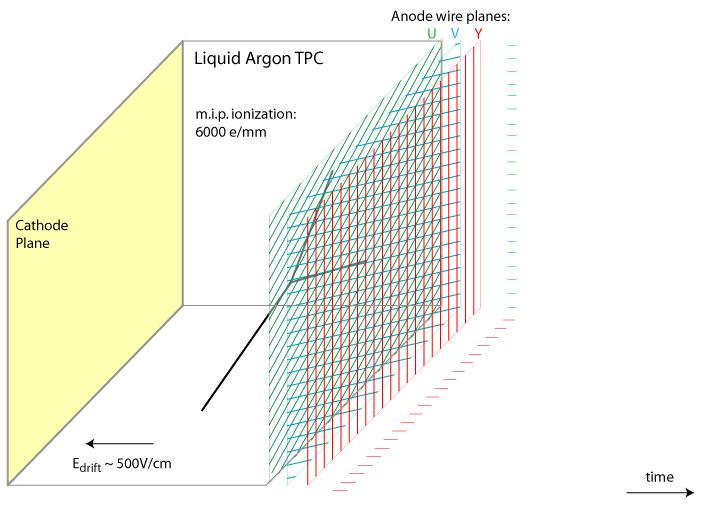
\includegraphics[width=0.9\textwidth]{signal-0.png}
	\caption{Liquid Argon TPC with wire readout: principle of operation}
	\label{fig:signal-0}
\end{figure}

The Liquid Argon Time Projection Chamber (LArTPC) is in essence a specially instrumented ionization chamber. Charges (electrons and positive ions)
created due to passage of ionizing particles through the sensitive medium (argon in this case) are subject to the effect of a uniform electrostatic
field which is created in Liquid Argon by a system of cathode and anode electrodes, which causes them to move (drift) along the field lines.
If there is an additional electrode within the Liquid Argon volume in the vicinity of the drifting charge, there will be a signal induced on it. Multiple such
electrodes (sensors) provide means for spatial characterization of the ionization charge distribution in the sensitive volume (which for example may
correspond to a particle track). Importantly, the shape of the signals on the electrode vs time is used to measure charge localization along the drift
direction (hence the term ``Time Projection Chamber''). For example, ionization electrons which are closer to the collection electrode will arrive to it sooner than
more distant ones, therefore time evolution of the signals on the affected wires will reflect distribution of the charge along the drift axis.

Current design of large scale LArTPC devices features planar arrays of wire electrodes supported by
rectangular frames. Such design contains an essential element called \textit{Anode Plane Assembly} (APA), which includes the ``collection plane'' (anode)
and two planes of sensor wires, called ``induction planes'', oriented at stereo angles with respect to each other and the collection plane.
Due to stereo angles, such arrangement allows for 2D measurement of the charge density distribution in the APA plane.
This is illustrated in Fig.~\ref{fig:signal-0}, which schematically shows the drift volume (to the left), the induction planes ``U'' and ``V'' and
the collection plane ``Y''. An important feature of such arrangement is that the \textit{same drifting charge} is measured three times as it
is detected by the three wire planes. This is further illustrated in Fig.~\ref{fig:3projections} as a schematic of drifting charge creating signals on wires,
represented conceptually as a view along the direction of the drift.

\begin{figure}[h!]
	\centering
	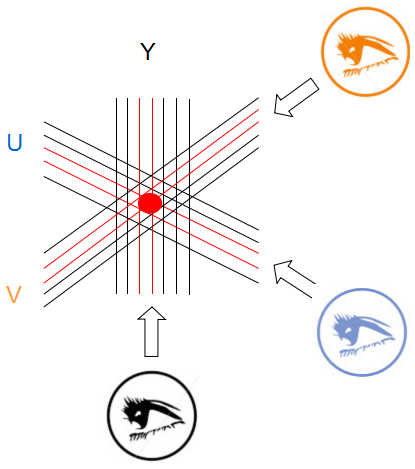
\includegraphics[width=0.65\textwidth]{uvy_2.png}
	\caption{Three projections of an object in a TPC with wire-based readout}
	\label{fig:3projections}
\end{figure}

Using just three projections to reconstruct an extended object (ionization charge density) presents challenges for event reconstruction.
Reliability and thorough characterization of the algorithms employed in this area will be critical for the systematics and other performance characteristics of DUNE.

There are a few approaches currenlty in development for event reconstruction. The ``Pandora'' toolkit (\ref{sec:pandora}), which
originated as R\&D for fine-grained calorimetry at ILC~\cite{pandora}, is being adopted to reconstruct LArTPC events.
In addition, there is a ``projection matching algorithm'' which will be used for test-beam studies with protoDUNE detector.

There is also a promising toolkit under development (called ``Wire Cell'') based on a different approach.
It performs three-dimensional imaging of events using the principles commonly applied in tomography.
As is frequently the case in tomographic reconstruction with sparse data, this may require the use memory- and CPU-intensive computing platforms.
It is likely that meeting the demands of such calculations will require adopting emerging technologies that are now becoming more common in
HEP, such as GPU or other co-processor acceleration and/or massively parallel systems such as HPC facilities.

\subsection{Pandora}
\label{sec:pandora}
 Pandora is a toolkit for implementing pattern recognition algorithms for fine-grain detectors, based on the so-called ``particle flow'' approach~\cite{pandora}.
It was conceived as a way to improve resolution of calorimetric measurements by taking advantage of the detector granularity. Pandora incorporates a
number of algorithms for different stages of event reconstruction, such as clustering algorithm, topological association algorithms, track-cluster association
algorithms and others, while providing a framework to utilize and manage these components. The framework also deals with memory management
and is designed to minimize external dependencies.

Pandora was adopted for event reconstruction in LBNE and now continues as a DUNE effort. It has been incorporated into the LArSoft sofware toolkit
as a package.



\subsection{Wire Cell}
\label{sec:wirecell}
\subsubsection{The Inverse Problem}

The LArTPC acts an imaging device, i.e. the physics information about the processes taking place in the detector volume is extracted by
analysing the 3D structures (images) of ionization patterns produced by particles participating in these processes. The only source of information
available for reconstruction of these images are amplitudes of signals coming from the wires in (U,V,Y) recorded as a function of time
as described above. It follows that the event reconstruction problem in DUNE TPC is a fairly typical case of the \textit{Inverse Problem},
where a 3D structure must be calculated based on a set of observables.

Because of time quantization inherent in operation of ADC, the 3D image effectively becomes an assembly of 2D slices.
In a given time slice, the 2D charge density distribution is observed via three different projections along the axes (U,V,Y) (see Fig.~\ref{fig:3projections}).
There is substantial similaritiy between this type of inverse problem and Computed Tomography (CT) with limited projection data. This similarity becomes even more prominent as we observe that in a
given slice the charge signals on wires are essentially linear integrals of the 2D charge density along each of the three observation axes. Common with many tomographic applications, the reconstruction strategy
then consists of calculating patterns in each 2D slice and then combining them into a full 3D structure. There are many event types and topologies
in DUNE, one example of a simulated neutral-current event in presented in Fig.~\ref{fig:ncc-example-1}.

\begin{figure}[h!]
	\centering
	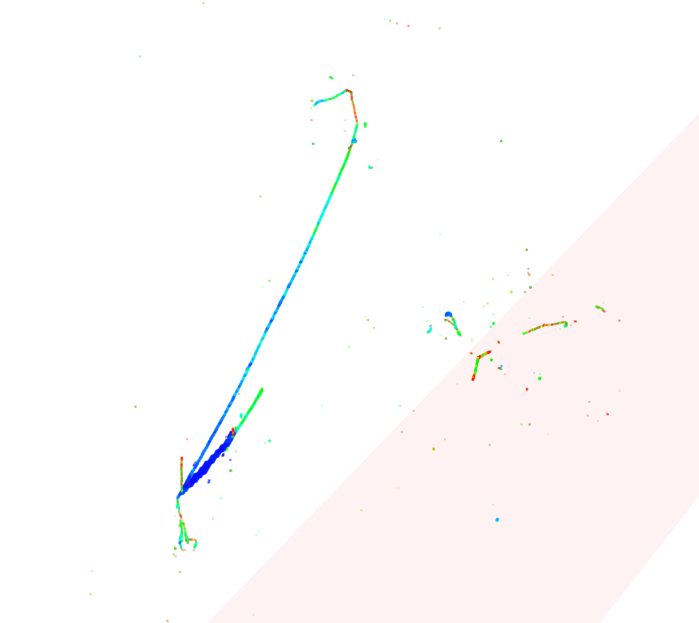
\includegraphics[width=0.7\textwidth]{ncc-example-1.png}
	\caption{An example of a neutrino-induced reaction in Liquid Argon ( simulation)}
	\label{fig:ncc-example-1}
\end{figure}

It's easy to see that (again, similar to majority of tomographic application) the reconstruction problem in DUNE is an ill-posed one,
due to the very limited set of just three observation angles. At the most basic level, this issue
manifests itself as ``ghost hits'' (well known in HEP), which is an ambiguity inherent in stereo
projection measurements.

The ``Wire Cell'' approach to this problem is based on the following:
\begin{itemize}
\item ``Voxelization'' of the TPC volume by treating each 2D slice as a tessellation (i.e. consisting of polygon-shaped tiles).

\item Solving an optimization problem which maximizes the likelihood of a given configuration of tiles (with charge associated with them) producing the observed signal distribution on the wires.

\item In reference to the optimization problem described above: regularization based on testing hypotheses about the object topology, e.g. that it's a track in a given portion of the volume. For example, cells in adjacent time slices can be tested for proximity in 2D.
\end{itemize}

To make this approach possible, there is one prerequisite that must be met, and that is a precise measurement of charge on each wire. This involves
proper calibration of the detector as well as solution of yet another inverse problem -- deconvolution of the detector and electronics reponse while
reconstructing the original shape of the charge signal. This is done in conditions of non-zero noise and involves applicaiton of digital filtering techniques.

\subsubsection{Wire Cell Components}
The flow of data in Wire Cell is presented in Fig.~\ref{fig:wirecell-diagram} in~\ref{sec:wc-diagram}.
Full description of Wire Cell is  beyond the scope and size limitations of this document,
so presented below is an annotated list of those elements of the data flow (see the diagram for specific
names) which are significant and/or present most computational challenges.
\begin{description}
\item[Slicer:] takes one "time frame" or a "readout" of raw data from DAQ (or simulated source)
and separates it in time bins.  Each bin contains ADC values for all the channels
(i.e. wires) with signal above a certain threshold that span the time bin.
	
\item[Cell Finder:] takes as a time bin and identifies ``cells'' (groups of adjacent tiles).
	
\item[Optimization Solver (``Matrix Solver''):] optimizes the likelihood of the charge contained in contiguous groups of cells
with respect to producing the observed signals on wires, utilizing a model where this relationship is expressed as a matrix.
	
\item[Clustering:] aggregates groups of cells over multiple time bins, thus creating 3D objects (``clusters'').
	
\item[Tracking:] connects clusters according to certain geometry rules, forming track candidates
	
\item[PID:] determines the type of particle based on ionization pattern, as defined by
charge depositions along the particle trajectory
\end{description}

\noindent
Elements listed above are computationally complex for a number of different reasons. For example,
the \textit{Cell Finder} performs a search on an array of tiles and given the large number
of those may face a combinatorial challenge. The \textit{Matrix Solver} has to solve an optimization
problem involving a sparse matrix. The \textit{Tracking} component has again to find relations
between multiple pieces of data based on applications of certain rules.
\newpage
\subsubsection{Wire Cell Diagram}
\label{sec:wc-diagram}
%\newpage
\begin{figure}[h!]
	\centering
	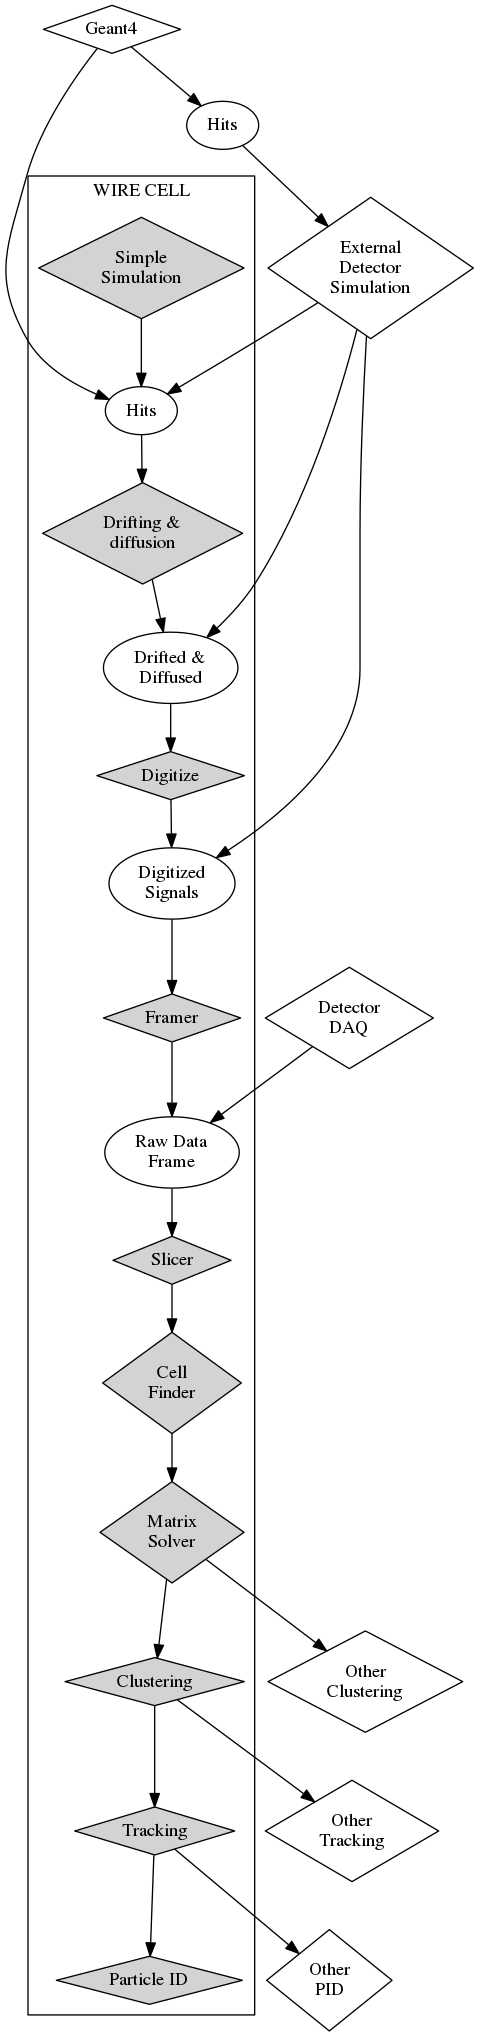
\includegraphics[height=0.8\textheight]{wirecell-dataflow-conceptual.png}
	\caption{Components of Wirecell Reconstruction Software}
	\label{fig:wirecell-diagram}
\end{figure}


\newpage